\documentclass[12pt]{exam}
\usepackage[utf8]{inputenc}		% Caracteres latinos
\usepackage[spanish]{babel}		% Idioma español
\usepackage{geometry}			% Organizar el documento
\usepackage{graphicx}			% Incluir gráficos
\usepackage{makecell}			% Para personalizar las celdas de una tabla
\usepackage{subcaption}
\usepackage[nohdr]{mathexam}	% Añadimos el paquete mathexam (sin header)
\usepackage{amsmath}
\usepackage{amsfonts}
\usepackage{amssymb}
\usepackage{mathtools}
\usepackage{float}

\usepackage{tikz,pgfplots}
\usepgfplotslibrary{polar}
\usepackage[shortlabels]{enumitem}
 \renewcommand{\baselinestretch}{1.5}
\usepackage{mathtools}
\usepackage{bm}
\usepackage{esvect}
\usepackage[fleqn]{mathtools}
\usepackage{relsize}
\usepackage{multirow}
\usepackage{multicol}
\usepackage[document]{ragged2e}
 \usepackage{textpos}
\usepackage{tcolorbox}
\usepackage{hyperref}


\geometry{
	a4paper,                    % Tamaño del documento
	hmargin = {1.7cm, 1.7cm}, 	% Margen horizontal izquierdo, derecho
	vmargin = {1cm, 1cm},	    % Margen vertical superior, inferior
	headsep = 4mm,				% Separación entre el encabezado y el texto
	head = .2cm,				% Tamaño del encabezado
	% marginparsep = 5mm, 		% Seperación entre las notas y el texto
	% marginpar = 1.5cm,		% Tamaño de las notas
	includeall,                 % incluye el encabezado, footer y notas dentro del tamaño del documento
	nomarginpar,	            % Elimina las notas
	foot = 1cm,                 % Tamaño del footer
	twoside,                	% Habilita el modo de impresión a doble cara
}

\selectlanguage{spanish}       
\spanishdecimal{.}


\newcommand{\iuni}{\pmb{\hat{\imath}}}
\newcommand{\juni}{\pmb{\hat{\jmath}}}
\newcommand{\kuni}{\pmb{\hat{k}}}


% DOCUMENTO
\begin{document}

\centering


\Large 
\textbf{Tarea A}\\
\large 
Unidad 1: Integral de Riemann. Integrales dobles.\\
Flores Morán Julieta Melina \\
\normalsize
Fecha de entrega: 
Viernes 23/08/2024 durante la clase




\vskip10pt
\normalsize

\pointpoints{punto}{puntos}
\pointformat{\bfseries\boldmath(\thepoints)}
\vskip10pt

    
    \begin{questions}

     \question
 %Ejercicio 1 --------------------------------------------------------------------------------------------------------------------------------------------
         Usa una suma de Riemann con $m=n=2$ para estimar el valor de $\mathlarger{\iint}_R\text{sen}(x+y)dA$, donde $R=[0,\pi]\times[0,\pi]$. Elige los puntos muestra como las esquinas inferiores izquierdas.
    \begin{figure}[h]
      \centering
      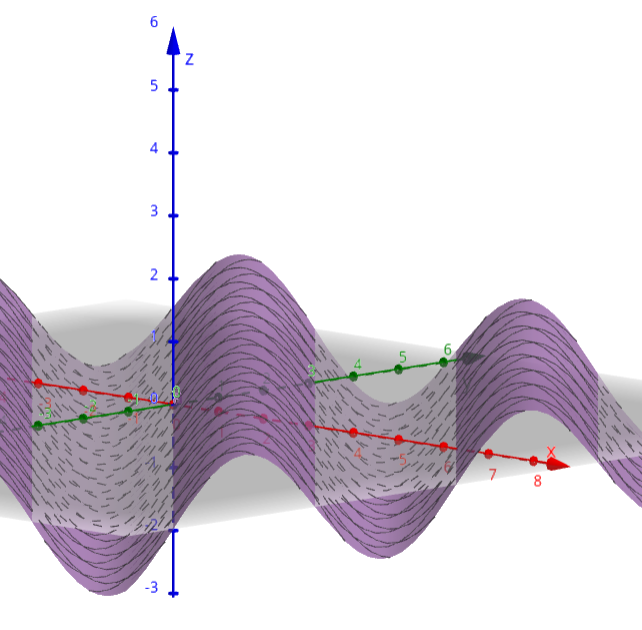
\includegraphics[width=0.3\textwidth]{./img/i1e1.png}
      \label{fig:sen1}
      \caption{$\sin{(x+y)}$}
    \end{figure}

    Sabemos que $\mathlarger{\iint}_{R}\text{sen}(x+y)dA = V  \approx \sum_{i=1}^{m}\sum_{j=1}^{n} f(x_{{ij}^*},y_{{ij}^*})\Delta A $.
  Lo que haremos será dividir la región R en m columnas y n renglones, así, la vertical queda dividida en $x_0=0, x_1=\frac{\pi}{2}, x_2=\pi$ y la vertical en $y_0=0, y_1=\frac{\pi}{2}, y_2=\pi$, por lo que al tomar la esquina izquierda de un cuadro $ij$ como punto muestra, tenemos que $(x_{{ij}^*},y_{{ij}^*}) = (x_{i-1}, y_{j-1})$
\begin{figure}[h]
      \centering
      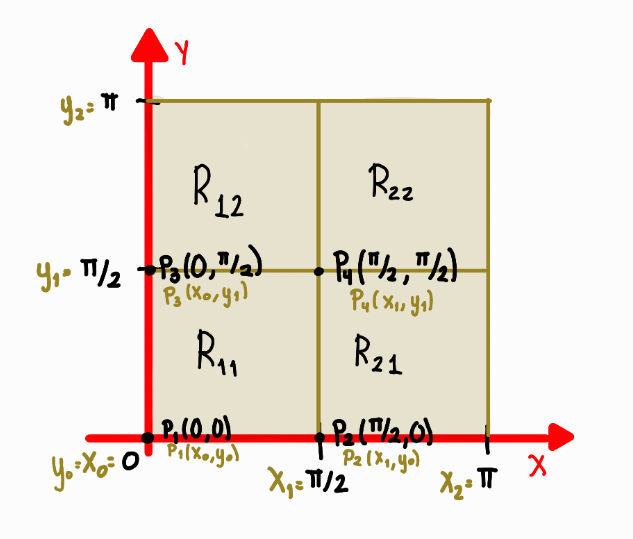
\includegraphics[width=0.5\textwidth]{./img/i2e1.png}
      \label{fig:región}
      \caption{Región de integración}
\end{figure}

Evaluando la función f(x,y) = sen(x+y) en cada punto muestra tenemos que:
\begin{itemize}
\item $f(x_0, y_0)= f(0,0) = sen(0+0) = 0$\\
\item $f(x_0,y_1) = f(0,\frac{\pi}{2}) = sen(0+\frac{\pi}{2}) = 1$\\
  \item $f(x_1, y_0) = f(\frac{\pi}{2},0) = sen(\frac{\pi}{2}+0) = 1$\\
\item $f(x_1, y_1) =  f(\frac{\pi}{2},\frac{\pi}{2}) = sen(\frac{\pi}{2}+\frac{\pi}{2}) = sen(\pi)= 0$\\
\end{itemize}
Lo último que necesitamos para sustituir es conocer $\Delta A$, que es el área de cada subregión $R_{ij}$, de ancho y largo miden $\frac{\pi-0}{2}$, por lo que $\Delta A =  \frac{\pi}{2}\frac{\pi}{2} = \frac{\pi^{2}}{4}$.\\
Desarrollando la suma de Riemann, tenemos que:

  \begin{align*}
    \int \int _R \sin{(x+y)} dA 
    &\approx \sum_{i=1}^{2}\sum_{j=1}^{2} \left[ f(x_{i-1},y_{j-1}) \cdot  \frac{\pi^2}{4} \right] \\
    &= \frac{\pi^2}{4} \left[ \sum_{i=1}^{2}\sum_{j=1}^{2} f(x_{i-1},y_{j-1}) \right] \\
    &= \frac{\pi^2}{4} \left[f(x_0,y_0)+f\left(x_0,y_1\right)+f\left(x_1,y_0\right)+f\left(x_1,y_1\right) \right] \\
    &= \frac{\pi^2}{4} \left(0+1+1+0 \right) \\
    &= \frac{\pi^2}{4}  \left(2 \right) = \frac{2\pi^2}{4}= \frac{\pi^2}{2} 
  \end{align*}

De esta manera, concluimos que, $\boldsymbol{\int \int _R \sin{(x+y)} dA \approx \frac{\pi^2}{2}}$
%Ejercicio 2---------------------------------------------------------------------------------------------------------------------------------------------

    \question
     En la siguiente figura se muestra un mapa de curvas de nivel para la función $f(x,y)$. Usa la Regla del Punto Medio con $m=n=2$ para estimar el valor de $\mathlarger{\iint}_Rf(x,y)dA$ en la región $R=[0,4]\times[0,4]$. 
     \begin{center}
         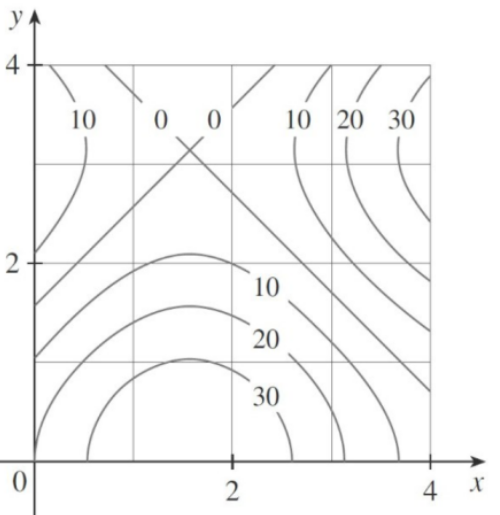
\includegraphics[scale=.35 ]{img/i1e2.png}
     \end{center}

 La regla del Punto Medio para integrales dobles nos dice que: $$ \mathlarger{\iint}_Rf(x,y)dA \approx \sum_{i=1}^{m} \sum_{j=1}^{n} f\left(\overline{x}_i, \overline{y}_j\right) \Delta A$$
 donde \( \overline{x}_i \) es el punto medio de \([x_{i-1}, x_i]\) y \( \overline{y}_j \) es el punto medio de \([y_{j-1}, y_j]\).
 Por lo que tenemos que $\left(\overline{x}_i, \overline{y}_j\right) = \left(\frac{x_i+x_{i-1}}{2}, \frac{y_i+y_{i-1}}{2} \right)$. En el caso de esta región, que dividiremos en 2 columnas y 2 filas, es decir 4 subregiones, los puntos medios y la evaluación estimada de f(x,y) según el mapa de curvas de nivel   son los siguientes: \\
\begin{multicols}{3}
 \begin{itemize}
 \item $ \overline{x_1} = \frac{x_1 + x_0 }{2} = \frac{2+0}{2} = 1 $ \\
 \item $ \overline{x_2} = \frac{x_2 + x_{1} }{2}  = \frac{4+2}{2} = 3$  \\
 \item $ \overline{y_1} = \frac{y_1 + y_0}{2} = \frac{2+0}{2} = 1 $ \\
 \item $ \overline{y_2} = \frac{y_2 + y_1}{2} = \frac{4+2}{2} = 3$
 \end{itemize}

  \begin{itemize}
  \item $ \left( \overline{x_1}, \overline{y_1} \right)= (1,1) $ \\
  \item  $ \left( \overline{x_2}, \overline{y_1} \right)= (3,1) $ \\
  \item $ \left( \overline{x_1}, \overline{y_2} \right)= (1,3) $ \\
  \item  $ \left( \overline{x_2}, \overline{y_2} \right)= (3,3) $ \\
 \end{itemize}
\begin{itemize}
  \item $f(1,1) \approx 27 $ \\
  \item  $f(3,1) \approx 4 $ \\
  \item $ f (1,3) \approx 13 $ \\
  \item  $ f(3,3) \approx 18$ \\
 \end{itemize}
\end{multicols}


 
\begin{figure}[H]
    \centering
    \begin{subfigure}[b]{0.4\textwidth}
        \centering
        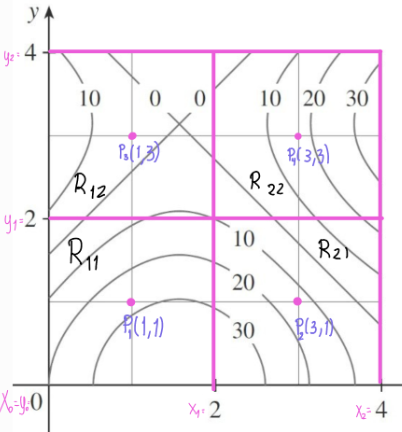
\includegraphics[width=\textwidth]{./img/i2e2.png}
        \caption{Puntos medios de la región R}
        \label{fig:mapa1}
    \end{subfigure}
    \hfill
    \begin{subfigure}[b]{0.4\textwidth}
        \centering
        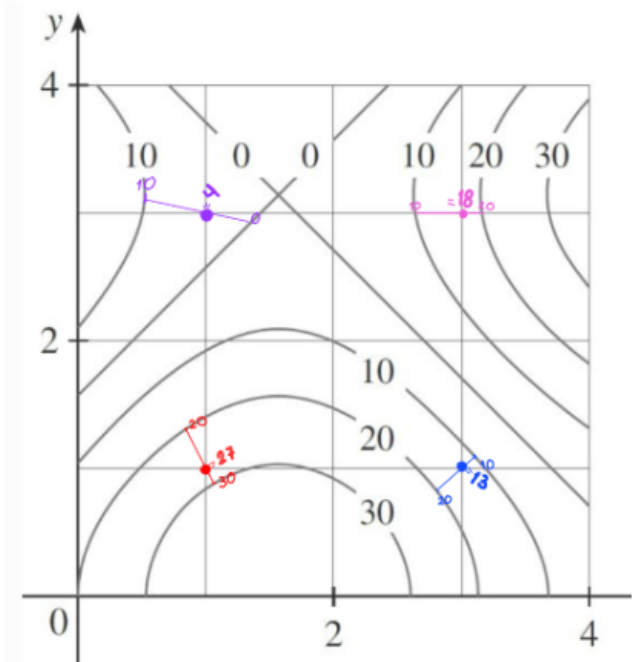
\includegraphics[width=\textwidth]{./img/i3e2.png}
        \caption{Estimaciones de la función f(x,y) en los puntos medios}
        \label{fig:mapa2}
    \end{subfigure}
    \caption{Región R }
\end{figure}


El área de cada subregión $R_{ij}$ es $\Delta A = 2\cdot2 = 4$. Ya con está información desarrollamos la suma de Riemann.

\begin{align*}
    \mathlarger{\iint}_Rf(x,y)dA
    &\approx \sum_{i=1}^{2} \sum_{j=1}^{2} \left[f\left(\overline{x}_i, \overline{y}_j\right) \cdot 4\right]\\
    &= 4 \left[\sum_{i=1}^{2} \sum_{j=1}^{2}f\left(\overline{x}_i, \overline{y}_j\right) \right]\\
    &= 4 \left[f(\overline{x}_i,\overline{y}_i)+f(\overline{x}_2,\overline{y}_1)+f(\overline{x}_1,\overline{y}_2)+f(\overline{x}_2,\overline{y}_2) \right]\\
    &= 4 \left[f(1,1)+f(1,3)+f(3,1)+f(3,3) \right]\\
    &= 4 \left(27+4+13+18\right) \\
    &= 4( 62)\\
    &= 248
  \end{align*}
Por lo tanto,  $\boldsymbol{\int \int _R f(x,y) dA \approx 248}$


%ejercicio 3 ---------------------------------------------------------------------------------------------------------------------------------------------
     \question
     Calcula las siguientes integrales iteradas.
     \begin{enumerate}[a)]
     \item $\mathlarger{\int}_0^2\mathlarger{\int}_0^{1}(2x+y)^8\,dx\,dy$
       \begin{figure}[h]
      \centering
      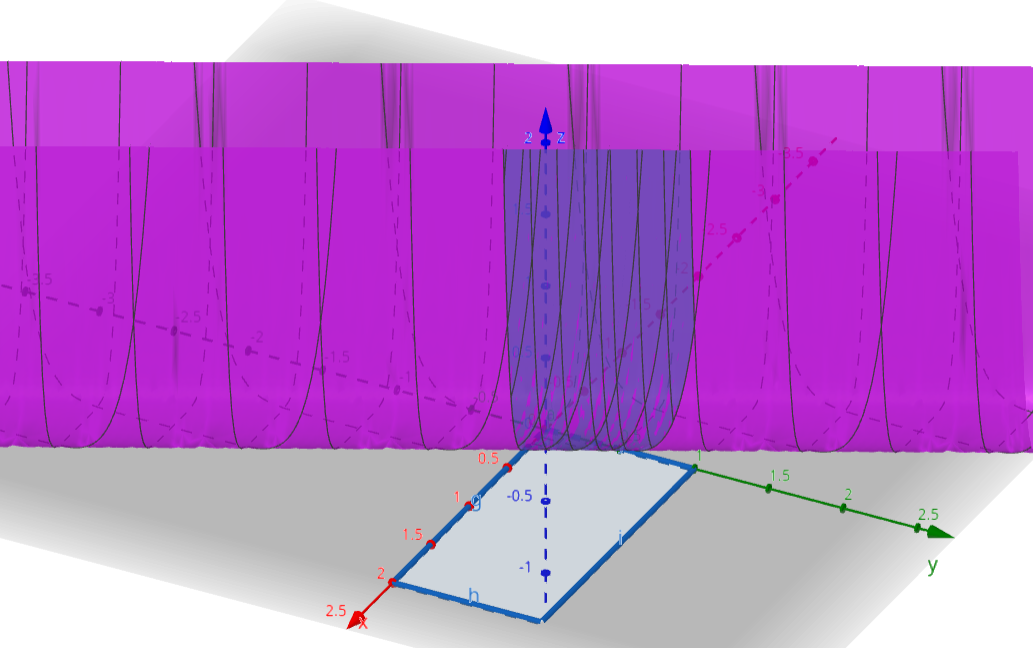
\includegraphics[width=0.5\textwidth]{./img/i1e3.png}
      \label{fig:región}
      \caption{La función $(2x+y)^8$ y la región de integración $[0,2]\times[0,1]$}
       \end{figure}

       Comenzamos con  $\mathlarger{\int}_0^{1}(2x+y)^8\,dx$ y resolvemos por sustitución.
       Sea $u = 2x+y$, $du = 2dx \rightarrow dx=\frac{1}{2}du$.Tenemos entonces que $\mathlarger{\int}_0^{1}(2x+y)^8\,dx = \frac{1}{2}\mathlarger{\int}_{u(0)}^{u(1)}u^8\,du = \frac{1}{2} = \frac{1}{2}\frac{u^9}{9}\Big| _{u(0)}^{u(1)} = \frac{u^9}{18}\Big| _{u(0)}^{u(1)}=  \frac{(2x+y)^9}{18}\Big| _{0}^{1} = \frac{(2(1)+y)^9}{18} -  \frac{(2(0)+y)^9}{18} =   \frac{(2+y)^9}{18} -\frac{y^9}{18}$. Por lo tanto :   $\mathlarger{\int}_0^2\mathlarger{\int}_0^{1}(2x+y)^8\,dx\,dy =  \mathlarger{\int}_0^2  \left[ \frac{(2+y)^9}{18} -\frac{y^9}{18}\right]  \,dy $ \\
        \begin{align*}
          &= \frac{1}{18} \left[  \mathlarger{\int}_0^2  \left[ (2+y)^9 -y^9\right]  \,dy \right] \\
          &= \frac{1}{18} \left[  \mathlarger{\int}_0^2  (2+y)^9 \,dy -  \mathlarger{\int}_0^2 y^9  \,dy \right] \\
          &= \frac{1}{18} \left[  \frac{(2+y)^{10}}{10} -  \frac{y^{10}}{10} \right]_{0}^{2} \\
           &=  \frac{(2+y)^{10}-y^{10}}{180} \Big|_{0}^{2} \\
          &=  \frac{(2+y)^{10}-y^{10}}{180} \Big|_{0}^{2} \\
          &=  \frac{(2+2)^{10}-2^{10}}{180} - \frac{(2+0)^{10}-0^{10}}{180} \\
          &=  \frac{4^{10}-2^{10}}{180} - \frac{2^{10}}{180} \\
          &=  \frac{2^{20}-2^{10}-2^{10}}{180}  \\
          &= \frac{2^{10} (2^{10}-1-1)}{180} = \frac{2^{10} (2^{10}-2)}{180} =\frac{2^{11} (2^{9}-1)}{180}  \\
            &= \frac{2^{10} (2^{9}-1)}{90} =   \frac{2^{9} (2^{9}-1)}{45} = 5814.0\overline{44}
        \end{align*}
        
       De esta manera, concluimos que : $\boldsymbol{\int_0^2 \int_0^1 (2x + y)^8 \, dx \, dy = 5814.\overline{44}}$
       %INTEGRAL B
     \item $\mathlarger{\int}_{0}^{ln\,2}\mathlarger{\int}_{0}^{ln\,5}e^{2x-y}\,dx\,dy$
        \begin{figure}[h]
      \centering
      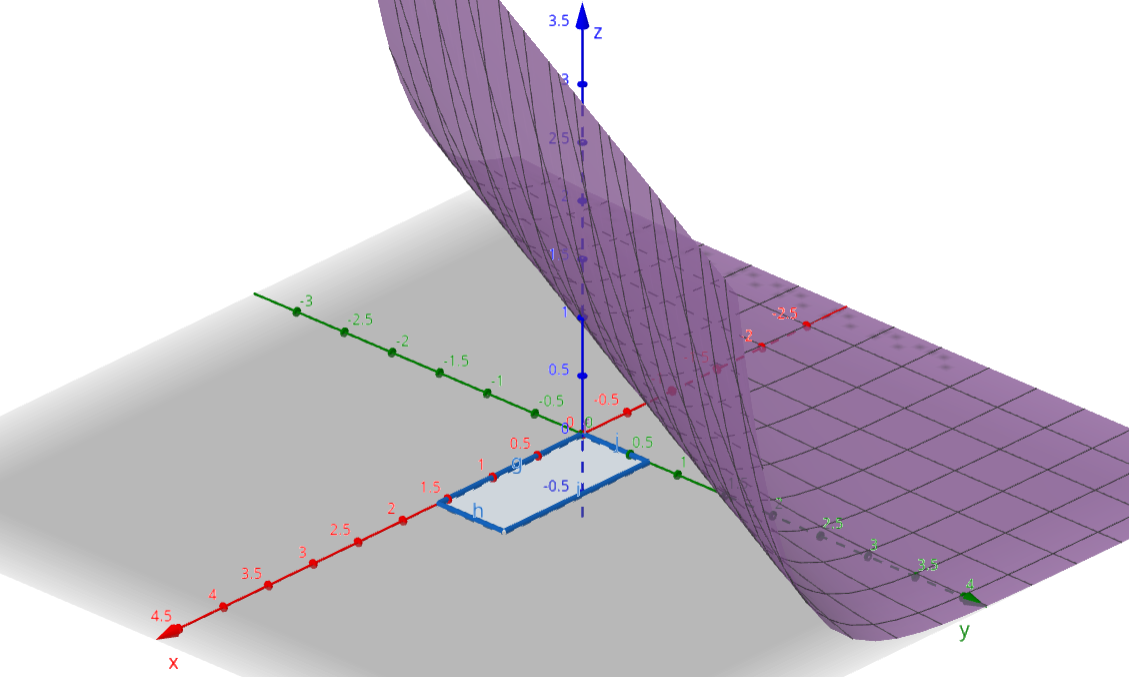
\includegraphics[width=0.5\textwidth]{./img/i2e3.png}
      \label{fig:región}
      \caption{La función $e^{2x-y}$ y la región de integración $[0,ln5]\times[0,ln2]$}
        \end{figure}
  
        Primero resolveremos $\mathlarger{\int}_{0}^{ln\,5}e^{2x-y}\,dx$. Integraremos por sustitución: Sea $u = 2x-y$, $du = 2dx \rightarrow dx=\frac{1}{2}du$ de esta manera tenemos que $\mathlarger{\int}_{0}^{ln\,5}e^{2x-y}\,dx =\frac{1}{2}\mathlarger{\int}_{u(0)}^{u(ln\,5)}e^{u}\,du = \frac{e^u}{2} \Big|_{u(0)}^{u(ln\,5)} =   \frac{e^{2x-y}}{2} \Big|_{0}^{ln\,5} =  \frac{e^{2(ln\,5)-y}}{2} -  \frac{e^{2\cdot0-y}}{2}$
         
         \begin{align*}
           &=  \frac{e^{2(ln\,5)-y}-e^{-y}}{2} \\
           &= \frac{e^{(ln\,5^2)}\cdot e^{-y}- \frac{1}{e^y}}{2} \\
           &= \frac{e^{(ln\,25)} \cdot \frac{1}{e^y} - \frac{1}{e^y}} {2} \\
           &= \frac{25 \cdot \frac{1}{e^y} - \frac{1}{e^y}} {2} \\
           &= \frac{ \frac{25-1}{e^y}} {2}  =  \frac{24}{2e^y} =  12e^{-y} 
         \end{align*}


         Ahora tenemos que  $\mathlarger{\int}_{0}^{ln\,2}\mathlarger{\int}_{0}^{ln\,5}e^{2x-y}\,dx\,dy = \mathlarger{\int}_{0}^{ln\,2}12e^{-y}\,dy $

         \begin{align*}
           &=  12 \mathlarger{\int}_{0}^{ln\,2}e^{-y}\,dy \\
           &= 12 \cdot -e^{-y} \Big|_{0}^{ln\,2} \\
           &= -12 \cdot e^{-y} \Big|_{0}^{ln\,2} \\
           &= -12e^{-ln\,2} - [ -12e^{0}] \\
           &= -12e^{ln\,2^{-1}} + 12\cdot 1 \\
           &=-12\cdot 2^{-1} + 12 \\
           &=-12\cdot \frac{1}{2} + 12 =-6+12 = 6   \\
         \end{align*}
         
     \end{enumerate}
     
     Por lo tanto, $\boldsymbol{\int_0^{ln2} \int_0^{ln5} e^{2x-y}\,dx\,dy  = 6}$
     
%Ejercicio 4 ---------------------------------------------------------------------------------------------------------------------
    \question 
    Un cilindro recto no circular tiene su base $D$ en el plano $xy$ y está acotado superiormente por el paraboloide $z=x^2+y^2$. El volumen del sólido es $$V=\mathlarger{\int}_0^1\mathlarger{\int}_0^{y}(x^2+y^2)\,dx\,dy + \mathlarger{\int}_1^2\mathlarger{\int}_0^{2-y}(x^2+y^2)\,dx\,dy$$ 
    Dibuja la región D y expresa el volumen como una sola integral iterada con el orden de integración invertido. Finalmente evalúa la integral para encontrar el volumen.    \\
    Podemos apreciar que la región de integración D esta descrita como una región de Tipo II donde y es delimitada por constantes y x entre funciones. La región de integración  $D =\{(x,y)| 0\leq y \leq 1, 0 \leq x \leq y\} \cup \{(x,y)| 1 \leq y \leq 2, 0 \leq x \leq 2-y\} $. Se ve de la siguiente manera: \\
    
  \begin{figure}[H]
    \centering
    \begin{subfigure}[b]{0.4\textwidth}
       \centering
      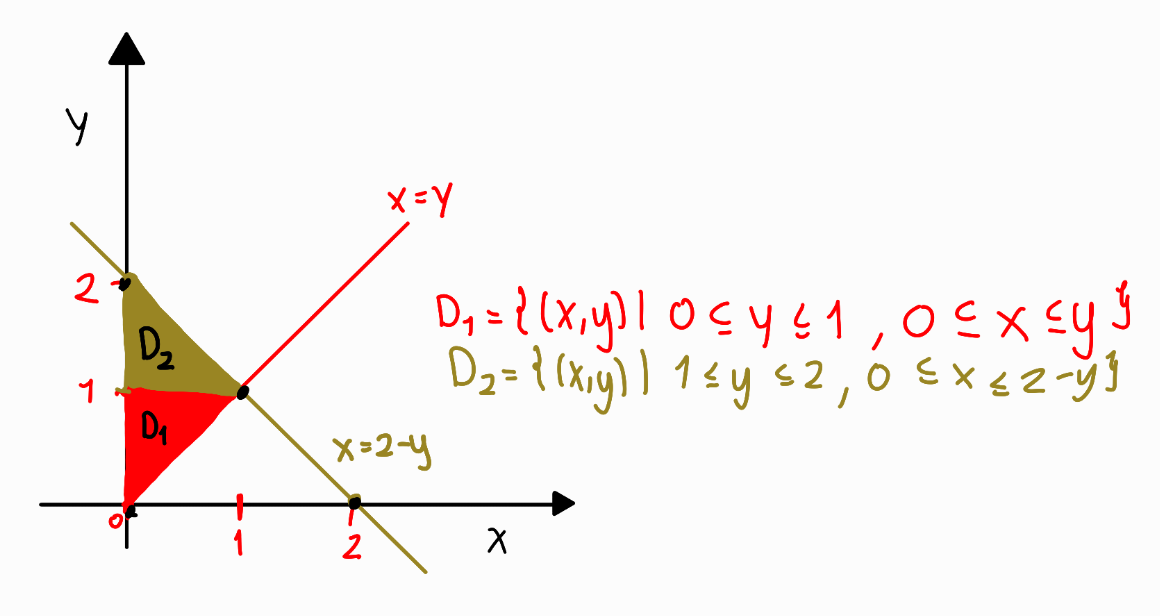
\includegraphics[width=1.5\textwidth]{./img/i1e4.png}
      \label{fig:región}
      \caption{\textbf{Dibujo de la región D}}
    \end{subfigure}
    \hfill
    \begin{subfigure}[b]{0.4\textwidth}
        \centering
        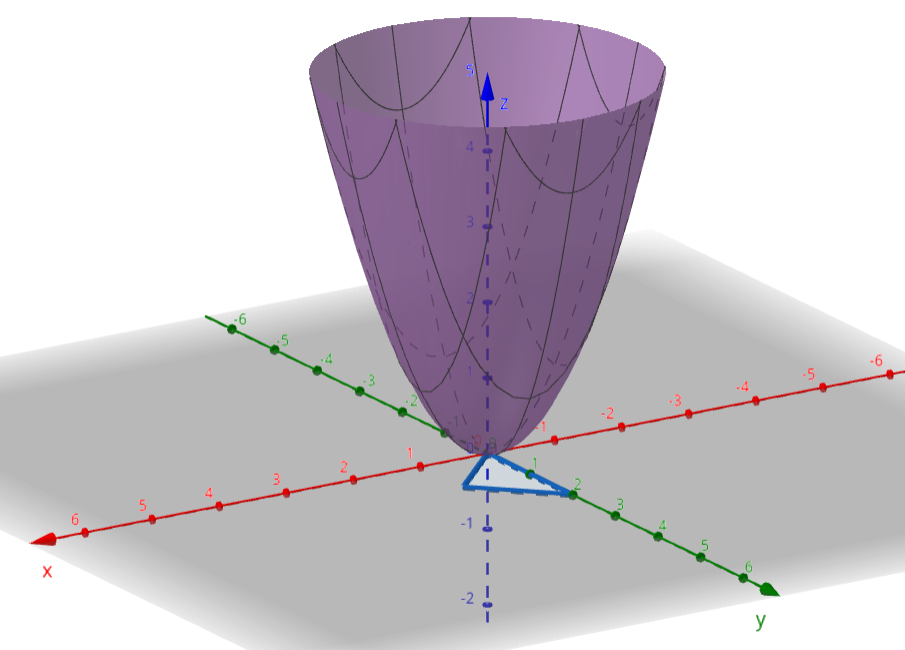
\includegraphics[width=\textwidth]{./img/i2e4.png}
        \caption{Función $z=x^2+y^2$ y la región de integración D}
        \label{fig:mapa2}
    \end{subfigure}
  \caption{Visualización }
  \end{figure}
  
    
       Podemos reescribir la región como una región de Tipo I donde x este acotado por constantes y y por funciones. Vemos en la imagen que x va de 0 a 1 y que y está entre x=y y x=2-y, en términos de x, y=x y y=2-x.\\
       Así, tenemos que $D=\{ (x,y)| 0\leq x \leq1 , x\leq y \leq 2-x\}$. Así podemos expresar el volumen de la siguiente forma con una sola integral iterada:\\
\[
    V=\mathlarger{\int}_0^1\mathlarger{\int}_0^{y}(x^2+y^2)\,dx\,dy + \mathlarger{\int}_1^2\mathlarger{\int}_0^{2-y}(x^2+y^2)\,dx\,dy = \boldsymbol{ \int_0^1\int_{x}^{2-x}(x^2+y^2)\,dy\,dx}
    \]
    Y resolvemos:
    \begin{align*}
      \mathlarger{\int}_0^1\mathlarger{\int}_{x}^{2-x}(x^2+y^2)\,dy\,dx & =  \mathlarger{\int}_0^1 \left[x^2 y + \frac{y^3}{3}\right]_x^{2-x}\,dx \\
      &=  \mathlarger{\int}_0^1 \left[x^2 (2-x) + \frac{(2-x)^3}{3} - \left( x^2 x + \frac{x^3}{3}\right)  \right] \,dx \\
      &=  \mathlarger{\int}_0^1 \left[2x^2-x^3+ \frac{(2-x)^3}{3} - x^3- \frac{x^3}{3} \right] \,dx \\
      &=  \mathlarger{\int}_0^1 \left[2x^2+ \frac{(2-x)^3}{3}-\frac{x^3}{3} - \frac{6x^3}{3} \right] \,dx \\
      &=  \mathlarger{\int}_0^1 \left[2x^2+ \frac{(2-x)^3}{3}-\frac{7x^3}{3} \right] \,dx \\
      &=  \mathlarger{\int}_0^1 \left[2x^2+ \frac{8-12x+6x^2-x^3}{3}-\frac{7x^3}{3} \right] \,dx \\
      &=  \mathlarger{\int}_0^1 \left[2x^2+ \frac{8}{3}-\frac{12x}{3}+\frac{6x^2}{3}-\frac{x^3}{3}-\frac{7x^3}{3} \right] \,dx \\
      &=  \mathlarger{\int}_0^1 \left[2x^2+ \frac{8}{3}-4x+2x^2-\frac{8x^3}{3} \right] \,dx \\
      &=  \mathlarger{\int}_0^1 \left[4x^2+ \frac{8}{3}-4x-\frac{8x^3}{3} \right] \,dx \\
       &=  \mathlarger{\int}_0^1 \left[4x^2+ \frac{8}{3}-4x-\frac{8x^3}{3} \right] \,dx \\
      &=   \left[4 \frac{x^3}{3}+ \frac{8x}{3}-\frac{4x^2}{2}-\frac{8x^4}{4\cdot 3} \right]_0^1 \,dx \\
      &=   \left[4 \frac{x^3}{3}+ \frac{8x}{3}-\frac{4x^2}{2}-\frac{8x^4}{12} \right]_0^1 \,dx \\
      &=   \left[ \frac{4x^3}{3}+ \frac{8x}{3}-2x^2-\frac{2x^4}{3} \right]_0^1 \,dx \\
      &= \frac{4x^3}{3}+ \frac{8x}{3}-2x^2-\frac{2x^4}{3} -0 \\
      &= \frac{4}{3}+ \frac{8}{3}-2-\frac{2}{3}=\frac{4}{3}+ \frac{8}{3}-\frac{6}{3}-\frac{2}{3} =\frac{4}{3} \\
    \end{align*}
Concluimos entonces que el volumen es : $ \boldsymbol{V = \frac{4}{3}} ~u^3 = 1.\overline{3}~u^3 $
%Ejercicio 5 ---------------------------------------------------------------------------------------------------------------------
     \question
       Encuentra el volumen de los sólidos con las siguientes características:
     \begin{enumerate}[a)]
     \item Acotado por la superficie $z=x\sqrt{x^2+y}$ y los planos $x=0$, $x=1$, $y=0$, $y=1$ y $z=0$.\\
       El área que buscamos está por debajo de $z=x\sqrt{x^2+y}$ y en la región que va de $x=0$ a $x=1$ y $y=0$ $y=1$.  Tenemos que la región de integración es $D=\{(x,y)|0 \leq x \leq 1, 0 \leq y \leq 1 \} =[0,1]\times[0,1]$.\\
      \begin{figure}[H]
    \centering
    \begin{subfigure}[b]{0.4\textwidth}
        \centering
        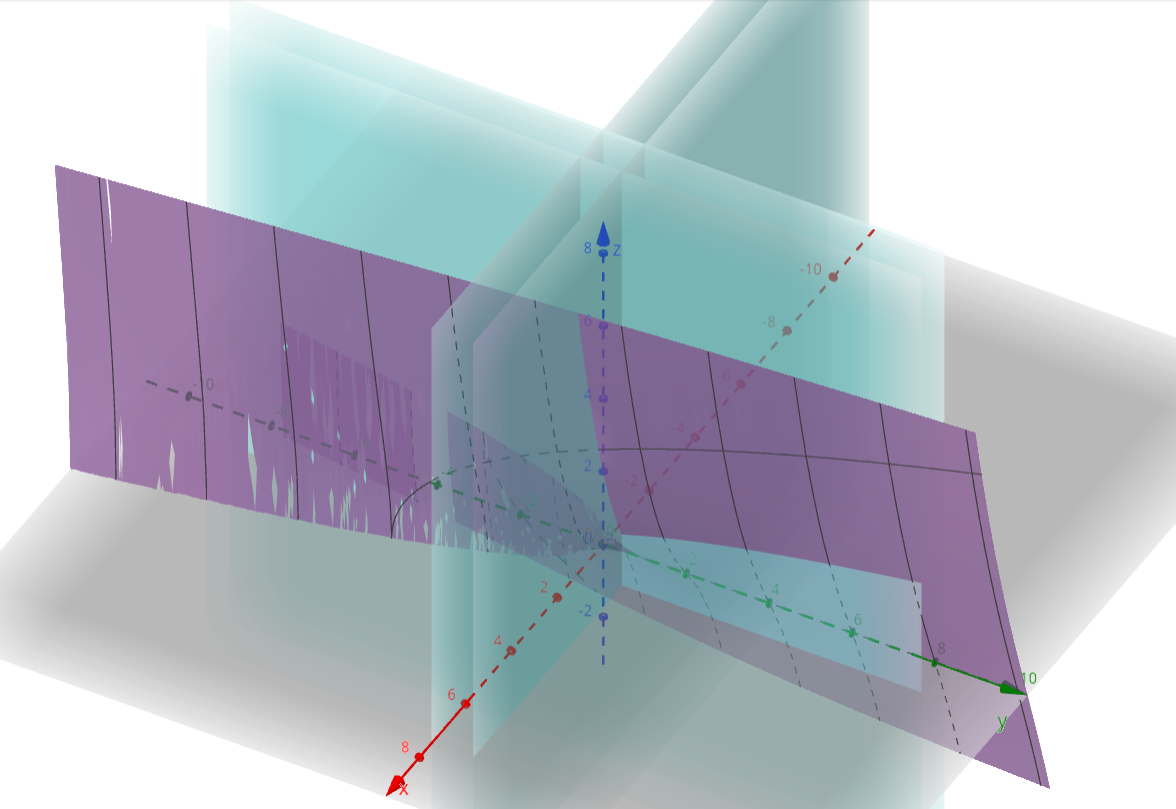
\includegraphics[width=\textwidth]{./img/i1e5.png}
        \caption{Planos y superficie que acotan al sólido}
        \label{fig:mapa1}
    \end{subfigure}
    \hfill
    \begin{subfigure}[b]{0.4\textwidth}
        \centering
        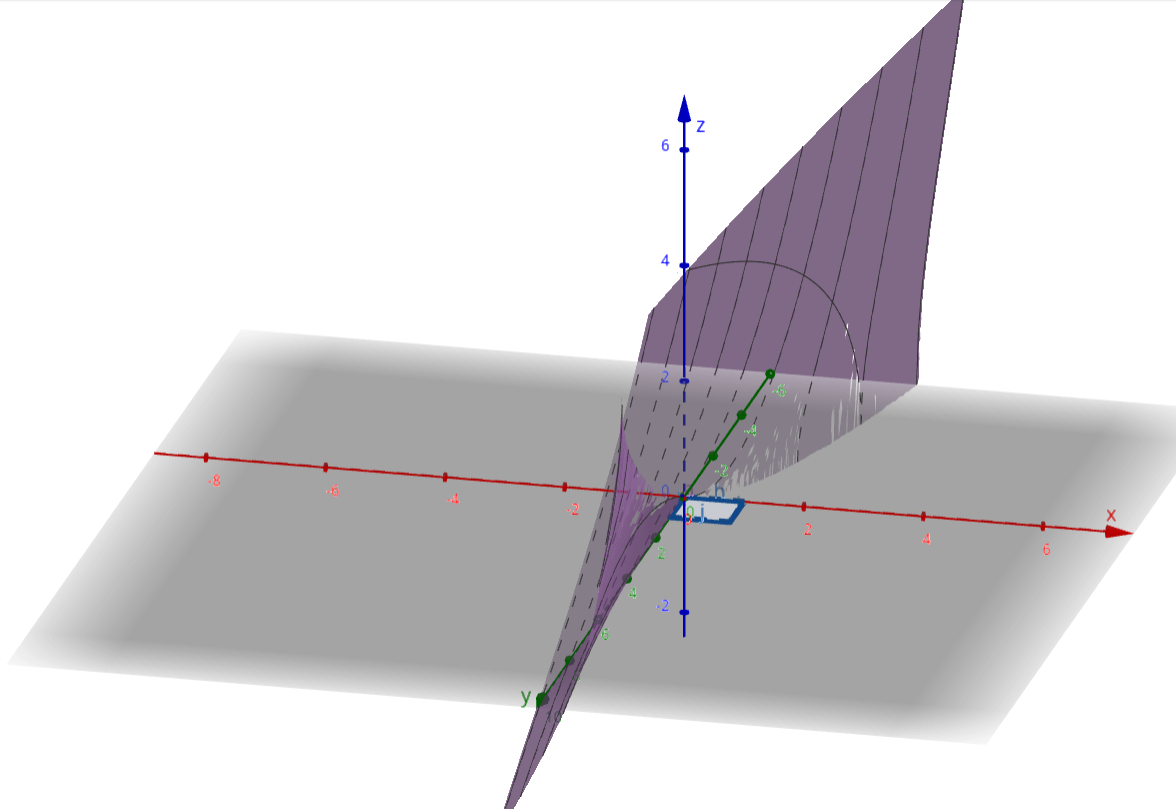
\includegraphics[width=\textwidth]{./img/i2e5.png}
        \caption{Superficie $z=x\sqrt{x^2+y}$ y la región de integración D}
        \label{fig:mapa2}
    \end{subfigure}
    \caption{Gráficas del área que acota al sólido}
      \end{figure}
      Así que la función que acota al sólido es  $z=x\sqrt{x^2+y}$ en el área D, por lo tanto,  $V = \mathlarger{\int}_0^1\mathlarger{\int}_0^{1}x \sqrt{x^2+y} \,dx\,dy $
      
      Primero integraremos $\mathlarger{\int}_0^{1}x \sqrt{x^2+y} \,dx$. Procederemos por sustitución, donde $u=x^2+y~\rightarrow ~ du=2xdx ~\rightarrow ~ \frac{du}{2}  = xdx$.
      Entonces tenemos que: 
     
    \begin{align*}
      \mathlarger{\int}_0^1\left(x\sqrt{x^2+y}\right)\,dx 
      &=  \frac{1}{2}\mathlarger{\int}_0^1\left(\sqrt{u}\right)\,du \\
      &=  \frac{1}{2}\mathlarger{\int}_{u(0)}^{u(1)}\left(u^{\frac{1}{2}}\right)\,du \\
      &=  \frac{1}{2} \left[ \frac{2}{3} u^{\frac{3}{2}} \right]_{u(0)}^{u(1)} \\
      &=  \left[ \frac{1}{3} (x^2 + y)^{\frac{3}{2}} \right]_{0}^{1} \\
      &=  \left[ \frac{1}{3} (1^2 + y)^{\frac{3}{2}} \right] -  \left[ \frac{1}{3} (0^2 + y)^{\frac{3}{2}} \right] \\
      &=  \frac{1}{3} (1 + y)^{\frac{3}{2}} -  \frac{1}{3}  + y^{\frac{3}{2}} = \frac{1}{3} \left( (1 + y)^{\frac{3}{2}} -  y^{\frac{3}{2}} \right)      
    \end{align*}

      Y sustituimos en $\mathlarger{\int}_0^1\mathlarger{\int}_0^{1}x \sqrt{x^2+y} \,dx\,dy$.
    \begin{align*}
      \mathlarger{\int}_0^1\mathlarger{\int}_0^{1}x \sqrt{x^2+y} \,dx\,dy
      &= \mathlarger{\int}_0^1\frac{1}{3} \left( (1 + y)^{\frac{3}{2}} -  y^{\frac{3}{2}} \right)  \,dy \\
      &= \frac{1}{3}\mathlarger{\int}_0^1 \left( (1 + y)^{\frac{3}{2}} -  y^{\frac{3}{2}} \right)  \,dy \\
      &= \frac{1}{3} \left[ \frac{2}{5}(1 + y)^{\frac{5}{2}} - \frac{2}{5} y^{\frac{5}{2}} \right]_{0}^{1} \\
      &= \frac{2}{15} \left (\left[(1 + 1)^{\frac{5}{2}} -  1^{\frac{5}{2}} \right] - \left[(1 + 0)^{\frac{5}{2}} -  0^{\frac{5}{2}} \right] \right) \\
      &= \frac{2}{15} \left (2^{\frac{5}{2}} -  1  - 1  \right) \\
      &= \frac{2}{15} \left (2^{\frac{4}{2}}\cdot2^{\frac{1}{2}} -  2  \right) \\
      &= \frac{2}{15} \left (4\cdot \sqrt{2} -  2  \right) \\
       &= \frac{8 \sqrt{2} - 4}{15} 
    \end{align*}

 Por lo tanto, el volumen del sólido es: $ \boldsymbol{V = \frac{8 \sqrt{2} - 4}{15} ~u^3 \approx 0.48758 ~u^3} $

 %%%%%%%%%%%%%%Ejercicio b %%%%%%%%%%%%%%%%%%%%%%%%%%%%%%%%%%%%%%%%
 
    
\item Encerrado por los cilindros $z=x^2$, $y=x^2$ y los planos $z=0$ y $y=4$.
  
  \begin{figure}[H]
    \centering
    \begin{subfigure}[b]{0.4\textwidth}
        \centering
        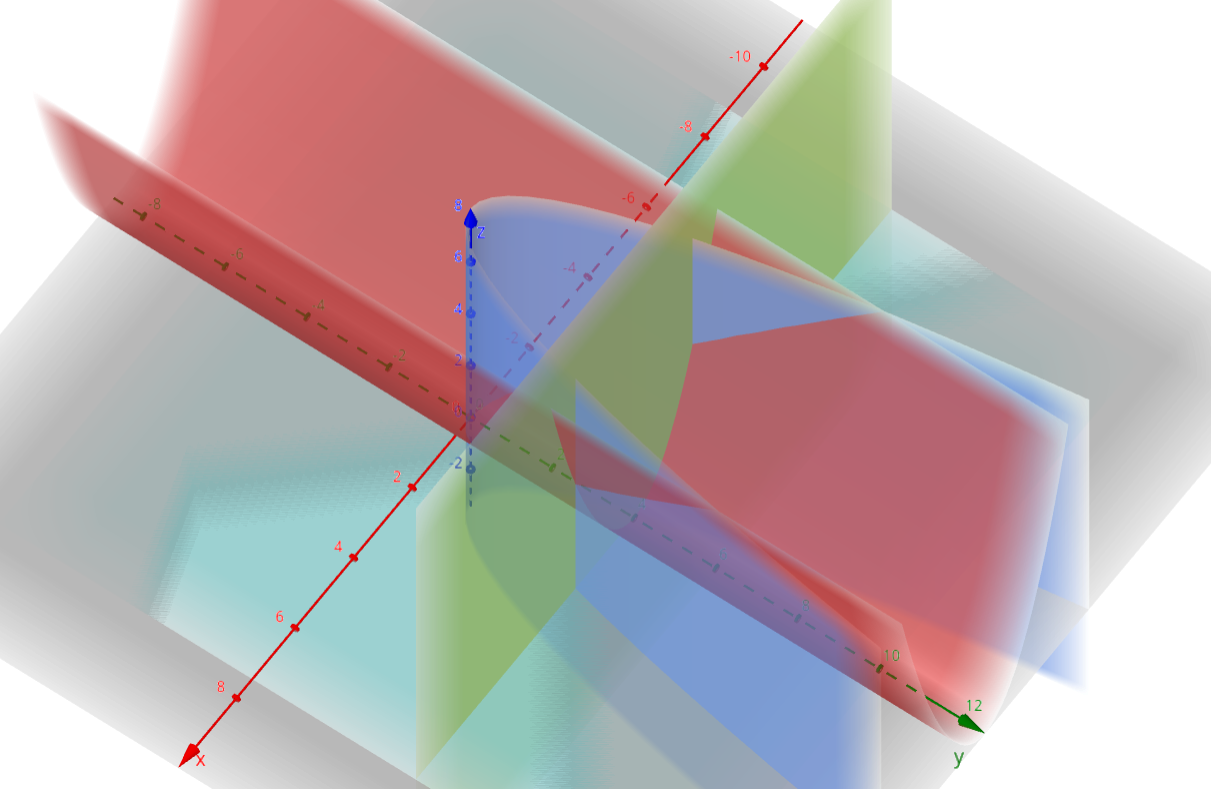
\includegraphics[width=\textwidth]{./img/i3e5.png}
        \label{fig:mapa1}
    \end{subfigure}
    \hfill
    \begin{subfigure}[b]{0.4\textwidth}
        \centering
        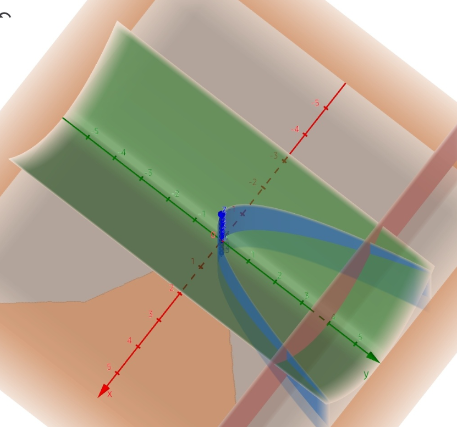
\includegraphics[width=\textwidth]{./img/i4e5.png}
        \label{fig:mapa2}
    \end{subfigure}
    \caption{Planos y cilindros que acotan al sólido}
      \end{figure}
  En este caso, podemos obtener el volumen del sólido tomando $z=x^2$ como la cota del sólido y viendo que el área de integración viene de describir el área entre $y=x^2$ y $y=4$ en el plano xy. Las funciones intersectan en dos puntos, en ambos $y=4$ y  $y=x^2 = 4 ~  \rightarrow x = \pm 2$, por lo tanto, los puntos en los que cortan son $(-2,4) \text{ y } (2,4)$.
  \begin{figure}[h]
      \centering
      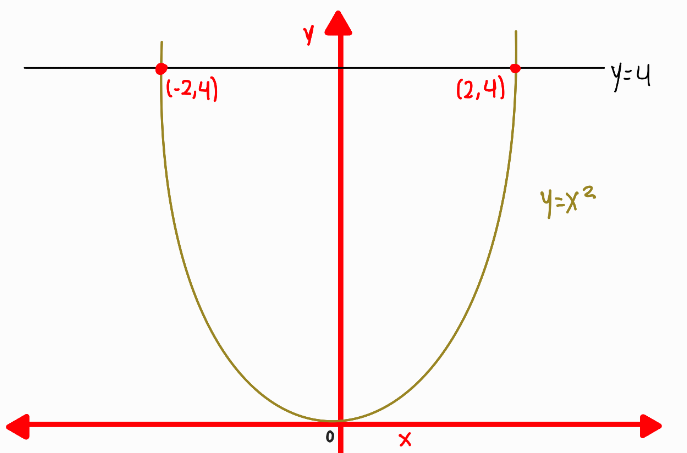
\includegraphics[width=0.5\textwidth]{./img/i5e5.png}
      \label{fig:regionxy}
      \caption{Región de integración}
  \end{figure}

  Podemos describir el área como una región Tipo I, es decir y simple donde y está acotada pro funciones y x por constantes. Vemos que x va de -2 a 2 y que y va de $y=x^2$ a $y=4$.
  Así la región de integración queda descrita de la siguiente manera: $D = \{(x,y)| -2\leq x \leq 2 , x^2 \leq y \leq 4\}$.
  De esta manera, tenemos que $V  = \mathlarger{\iint}_D x^2 \,dA =  \mathlarger{\int}_{-2}^2\mathlarger{\int}_{x^2}^{4}x^2 \,dy\,dx $. Y resolvemos para obtener el volumen.

  \begin{align*}
    \mathlarger{\int}_{-2}^2\mathlarger{\int}_{x^2}^{4}x^2 \,dy\,dx
    &= \mathlarger{\int}_{-2}^2 \left[ x^2 y \right]_{x^2}^{4} \,dx\\
    &= \mathlarger{\int}_{-2}^2 \left[ x^2 (4) \right] - \left[ x^2 (x^2) \right] \,dx\\
    &= \mathlarger{\int}_{-2}^2 \left[ 4x^2 -  x^4 \right] \,dx\\
    &=  \left[ \frac{4x^3}{3}-  \frac{x^5}{5} \right]_{-2}^2\\
    &=  \left[ \frac{4(2)^3}{3}-  \frac{(2)^5}{5} \right] -  \left[ \frac{4(-2)^3}{3}-  \frac{(-2)^5}{5} \right] \\
    &=  \frac{4(8)}{3}-  \frac{32}{5} -  \frac{4(-8)}{3} +  \frac{(-32)}{5}  \\
      &=  \frac{32}{3}-  \frac{32}{5} +  \frac{32}{3} -  \frac{32}{5}  \\
      &=  \frac{64}{3}-  \frac{64}{5} = \frac{320-192}{15} = \frac{128}{15}
    \end{align*}

  Por lo tanto, el volumen del sólido es $ \boldsymbol{V = \frac{128}{15} ~u^3 = 8.5\overline{3} ~u^3} $
     \end{enumerate}
     
%Ejercicio 6 ---------------------------------------------------------------------------------------------------------------------
     \question
     Evalúa la integral invirtiendo el orden de integración.
     \begin{enumerate}[a)]
     \item $\mathlarger{\int}_0^1\mathlarger{\int}_{3y}^3 e^{x^2}\,dx\,dy$ \\
       Con límites de la integral, podemos ver que la región de integración se describe como $D = \{ (x,y)| 3y \leq x \leq 3, 0 \leq y \leq 1 \}$, es decir, como una región $x$-simple, de tipo II. Y la podemos ver graficada de a siguiente forma:
       

        \begin{figure}[H]
      \centering
      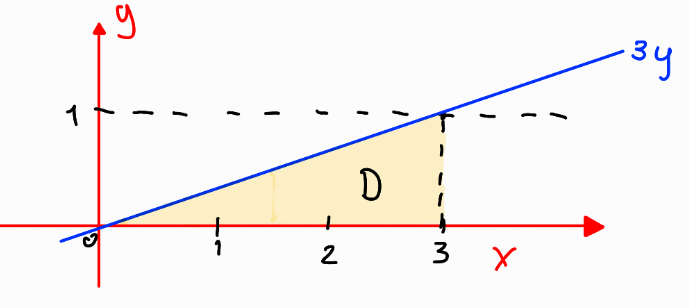
\includegraphics[width=0.5\textwidth]{./img/i1e6.png}
      \label{fig:región}
      \caption{La región de integración D}
        \end{figure}

 Podemos reescribirlo como una región de tipo I, es decir, $y$ -simple, donde $y$ vaya entre funciones y $x$ entre constantes. Por la imagen podemos observar que $x$ va de 0 a 3 y que $y$ va de 0 a $x=3y$ que reescrita en términos de $y$, sería $y= \frac{x}{3}$. Entonces otra manera de escribir la región D sería: $D= \{(x,y)| 0 \leq x \leq 3, 0 \leq y \leq \frac{x}{3} \}$. Gracias a esto, sabemos que:\\
        \[
        \mathlarger{\int}_0^1\mathlarger{\int}_{3y}^3 e^{x^2}\,dx\,dy = \mathlarger{\int}\mathlarger{\int_D}  e^{x^2} \,dA  = \boldsymbol{ \int_0^3\int_{0}^{\frac{x}{3}} e^{x^2}\,dy\,dx}
        \]

 Ya que hemos invertido el orden de integración, resolvemos.

 \begin{align*}
   \mathlarger{\int}_0^3\mathlarger{\int}_{0}^{\frac{x}{3}} e^{x^2}\,dy\,dx
   &= \mathlarger{\int}_0^3\left[  e^{x^2} y \right]_{0}^{\frac{x}{3}} \,dx \\
   &= \mathlarger{\int}_0^3\left[  e^{x^2} \frac{x}{3} \right] - \left[  e^{x^2} (0) \right] \,dx \\
   &= \mathlarger{\int}_0^3\left[  e^{x^2} \frac{x}{3} \right] \,dx \\
   &= \frac{1}{3} \mathlarger{\int}_0^3\left[  e^{x^2}x  \right] \,dx \\
 \end{align*}

 Procedemos por sustitución, sea $u = e^{x^{2}} ~ \rightarrow ~ du =  e^{x^{2}} 2xdx ~ \rightarrow ~ \frac{du}{2} = e^{x^{2}} xdx $, de esta forma:

\begin{align*}
  \frac{1}{3} \mathlarger{\int}_0^3\left[  e^{x^2}x  \right] \,dx
  &=  \frac{1}{3} \cdot  \frac{1}{2}  \mathlarger{\int}_{u(0)}^{u(3)}du \\
  &= \frac{1}{6} \left[ u \right]_{u(0)}^{u(3)} \\
  &= \frac{1}{6} \left[  e^{x^{2}} \right]_{0}^{3} \\
   &= \frac{ e^{3^{2}}  -  e^{0^{2}} }{6}  = \frac{ e^9  -  e^{0} }{6} =   \frac{ e^9  -  1 }{6}  \\
\end{align*}

Por lo tanto, $\boldsymbol{ \int_0^1\int_{3y}^3 e^{x^2}\,dx\,dy =   \int_0^3\int_{0}^{\frac{x}{3}} e^{x^2}\,dy\,dx = \frac{ e^9  -  1 }{6} \approx 1350.34732}$
       %%%%%%%%%%%%%%EJERCICIO B%%%%%%%%%%%%%%%%%%%%%%%%5
\item $\mathlarger{\int}_0^1\mathlarger{\int}_{\text{arcsen}\,y}^{\pi/2}\text{cos}(x)\sqrt{1+\text{cos}^2x}\,dx\,dy$ \\
  Por los límites de la integral podemos ver que la región de integración es de tipo II, pues se describió con $x$ entre funciones y $y$ entre constantes,así que es de la forma $D = \{ (x,y)| arcseny \leq x \leq \frac{\pi}{2} ,  ~ 0 \leq y \leq 1 \}$. Lo cual se puede visualizar de la siguiente manera:

 \begin{figure}[h]
      \centering
      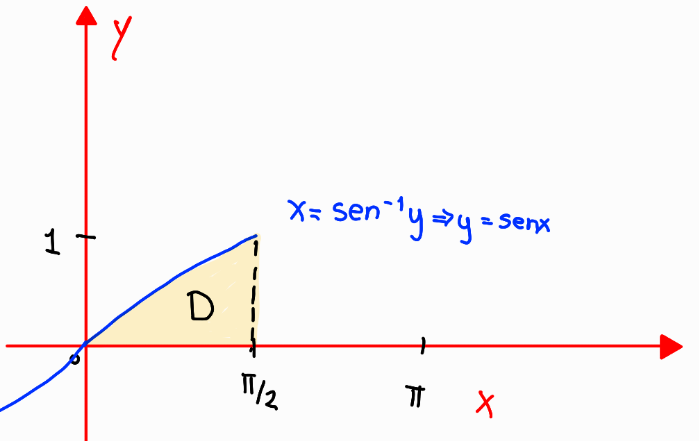
\includegraphics[width=0.5\textwidth]{./img/i2e6.png}
      \label{fig:región}
      \caption{La región de integración D}
 \end{figure}

 Podemos guiarnos en la imagen para describir la región como $y$-simple donde $y$ vaya entre funciones y $ x$ en contantes, observamos que $x$ va de $ 0 $ a $\frac{\pi}{2}$ y $y$ va de 0 a $\text{arcsen}\,y$, que reescrita en términos de $x$, será $x = \sen{y}$. Así que podemos describir está región de Tipo I como :  $D= \{(x,y)| 0 \leq x \leq \frac{\pi}{2}, 0 \leq y \leq \sen{x} \}$. Así vemos que entonces:
 \[
 \mathlarger{\int}_0^1\mathlarger{\int}_{\text{arcsen}\,y}^{\pi/2}\text{cos}(x)\sqrt{1+\text{cos}^2x}\,dx\,dy   = \boldsymbol{\int_0^{\frac{\pi}{2}}\int_{0}^{\sen{x}} \cos{x}\sqrt{1+\cos^2{x}} \,dy\,dx}
 \]

 Ahora evaluamos está integral:
 

\begin{align*}
  \mathlarger{\int}_0^{\frac{\pi}{2}}  \mathlarger{\int}_{0}^{\sen{x}} \cos{x}\sqrt{1+\cos^2{x}} \,dy\,dx
  &= \mathlarger{\int}_0^{\frac{\pi}{2}}  \left [ \cos{x}\sqrt{1+\cos^2{x}} y\right]_{0}^{\sen{x}} \,dx \\
  &= \mathlarger{\int}_0^{\frac{\pi}{2}}  \left [ \cos{x}\sqrt{1+\cos^2{x}} \sen{x} \right] - \left [ \cos{x}\sqrt{1+\cos^2{x}} (0) \right]  \,dx \\
  &= \mathlarger{\int}_0^{\frac{\pi}{2}}  \left [ \cos{x}\sen{x}\sqrt{1+\cos^2{x}}  \right] \,dx
\end{align*}
Procederemos por sustitución, sea $u = 1+\cos^2{x} ~ \rightarrow  ~ du = -2\cos{x}\sen{x}dx ~ \rightarrow  ~ -\frac{du}{2} = \cos{x}\sen{x}dx$. 

\begin{align*}
  \mathlarger{\int}_0^{\frac{\pi}{2}}  \left [ \cos{x}\sen{x}\sqrt{1+\cos^2{x}}  \right] \,dx
  &=  -\frac{1}{2}\mathlarger{\int}_{u(0)}^{u\left(\frac{\pi}{2}\right)}  \sqrt{u}  \,du \\
  &=  -\frac{1}{2}\mathlarger{\int}_{u(0)}^{u\left(\frac{\pi}{2}\right)}  u^{\frac{1}{2}}  \,du \\
  &=  -\frac{1}{2}\left[ \frac{2}{3}u^{\frac{3}{2}}  \right]_{u(0)}^{u\left(\frac{\pi}{2}\right)} \\
  &= \left[ -\frac{1}{3}( 1+\cos^2{x})^{\frac{3}{2}}  \right]_{0}^{\frac{\pi}{2}} \\
  &= \left[ -\frac{1}{3}\left( 1+\cos^2{\frac{\pi}{2}}\right)^{\frac{3}{2}}  \right] - \left[ -\frac{1}{3}( 1+\cos^2{0})^{\frac{3}{2}}  \right] \\
  &=  -\frac{1}{3}  \left( 1+\cos^2{\frac{\pi}{2}}\right)^{\frac{3}{2}}   + \frac{1}{3}( 1+\cos^2{0})^{\frac{3}{2}}   \\
  &= \frac{(1+1^2)^{\frac{3}{2}}  - (1+0^2)^{\frac{3}{2}} }{3} \\
  &= \frac{2^{\frac{3}{2}}  - 1 }{3} = \frac{2^{\frac{2}{2}} \cdot 2^{\frac{1}{2}} - 1 }{3} \\
  &= \frac{2 \sqrt{2} - 1 }{3}
\end{align*}
     \end{enumerate}

     Por tanto, tenemos que evaluando con los límites invertidos $\boldsymbol{ \int_0^{\frac{\pi}{2}}\int_{0}^{\sen{x}} \cos{x}\sqrt{1+\cos^2{x}} \,dy\,dx = \frac{2 \sqrt{2} - 1 }{3} \approx 0.60947} $
     
%Ejercicio 7 ---------------------------------------------------------------------------------------------------------------------
     \question
     Encuentra el volumen del sólido $S$ como la diferencia entre dos volúmenes. $S$ es el sólido encerrado por los cilindros parabólicos $y=1-x^2$, $y=x^2-1$ y las planos $x+y+z=2$, $2x+2y-z+10=0$.\\
     El sólido está acotado por las siguientes superficies y planos:

      \begin{figure}[H]
      \centering
      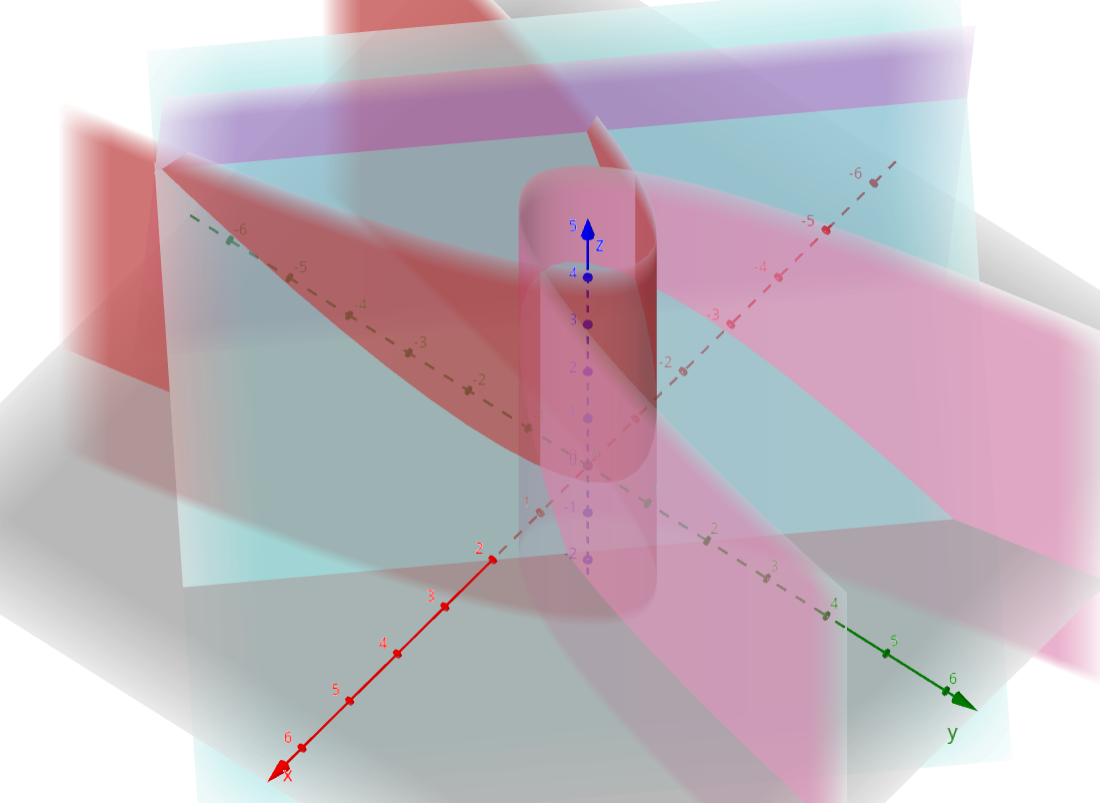
\includegraphics[width=0.5\textwidth]{./img/i1e7.png}
      \label{fig:región}
      \caption{Los cilindros y los planos que limitan a la superficie}
      \end{figure}
      Para ver el área de integración, veamos como se compartan nuestras funciones en el plano $xy$.
      \begin{itemize}
      \item $y=1-x^2$ es una parábola en el plano xy
      \item $y=x^2-1$ es una parábola en el plano xy, que intersecta con $y=1-x^2$ en el punto donde $1-x^2 = x^2-1 \rightarrow  1+1 = x^2+x^2 \rightarrow  2 = 2x^2 \rightarrow 1 = x^2 \rightarrow x = \pm 1  $
      \item $x+y+z=2$ en el plano $xy$, $z=0$.Entonces es la función $x+y=2 ~ \rightarrow ~ y=2-x$
        \item $2x+2y-z+10=0$, en el plano $xy$ $z=0$. Entonces es la función $2x+2y+10=0 ~ \rightarrow ~ 2x+10=-2y ~  \rightarrow x+5=-1y \rightarrow -x-5 =y $
      \end{itemize}
      Por lo anterior, el plano $xy$ se ve de la siguiente manera. La región de integración será la que este entre estas funciones, que es la región acotada por las parábolas:
      
    \begin{figure}[H]
      \centering
      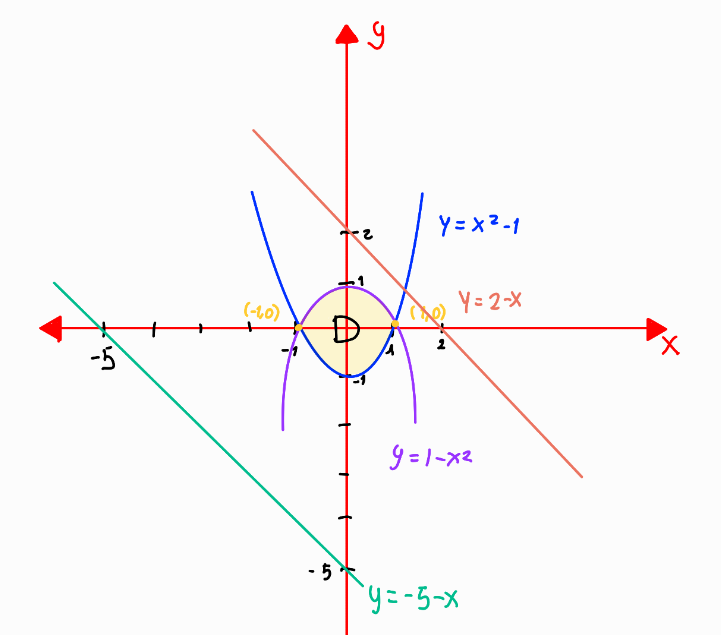
\includegraphics[width=0.5\textwidth]{./img/i2e7.png}
      \label{fig:región}
      \caption{La región de integración D}
    \end{figure}
    
    Así que podemos describir la región D como $y$-simple.  $D = \{ (x,y)| -1\leq x \leq 1, x^2 -1 \leq y \leq 1-x^2 \}$. Vemos que  $z =2-x-y $ $\leq$  $z = 2x+2y+10$ y como  el sólido $S$ está entre dos planos, podemos calcularlo como el volumen bajo  $z = 2x+2y+10$ menos el volumen bajo $z =2-x-y $. Así obtenemos que:
    \[
    V = \mathlarger{\int}_D \mathlarger{\int}_D 2x+2y+10  \,dA - \mathlarger{\int}_D \mathlarger{\int}_D 2-x-y  \,dA = 
    \]
     \[
     \mathlarger{\int}_{-1}^{1} \mathlarger{\int}_{x^2-1}^{1-x^2}[ 2x+2y+10 ] \,dy \,dx - \mathlarger{\int}_{-1}^{1} \mathlarger{\int}_{x^2-1}^{1-x^2} [ 2-x-y]  \,dy \,dx
     \]
     Y resolvemos:
     
     \begin{align*}
       V&= \mathlarger{\int}_{-1}^{1} \mathlarger{\int}_{x^2-1}^{1-x^2} 2x+2y+10  \,dy \,dx - \mathlarger{\int}_{-1}^{1} \mathlarger{\int}_{x^2-1}^{1-x^2}  2-x-y  \,dy \,dx  \\
       &=\mathlarger{\int}_{-1}^{1} \mathlarger{\int}_{x^2-1}^{1-x^2} 2x+2y+10 - [ 2-x-y]\,dy \,dx  \\
      & =\mathlarger{\int}_{-1}^{1} \mathlarger{\int}_{x^2-1}^{1-x^2} [2x+2y+10   - 2 + x +y] \,dy \,dx  \\
        &=\mathlarger{\int}_{-1}^{1} \mathlarger{\int}_{x^2-1}^{1-x^2} [3x+3y+8]\,dy \,dx  \\
       &=\mathlarger{\int}_{-1}^{1}  \left[ 3xy+\frac{3y^2}{2}+8y \right]_{x^2-1}^{1-x^2} \,dx  \\
        &=\mathlarger{\int}_{-1}^{1}  \left[ 3x(1-x^2)+\frac{3(1-x^2)^2}{2}+8(1-x^2) \right] - \left[ 3x(x^2-1)+\frac{3(x^2-1)^2}{2}+8(x^2-1) \right]  \,dx  \\
       & =\mathlarger{\int}_{-1}^{1}  3x(1-x^2)+\frac{3(1-2x^2+x^4)}{2}+8(1-x^2)- 3x(x^2-1)-\frac{3(x^4-2x^2+1)}{2}-8(x^2-1)   \,dx  \\
        &= \mathlarger{\int}_{-1}^{1}  3x-3x^3+\frac{3-6x^2+3x^4}{2}+8-8x^2- 3x^3+3x+\frac{-3x^4+6x^2-3}{2}-8x^2 + 8   \,dx  \\
       &= \mathlarger{\int}_{-1}^{1}  3x-3x^3+\frac{3}{2} - 3x^2+\frac{3x^4}{2}+8-8x^2- 3x^3+3x-\frac{3x^4}{2} +3x^2 - \frac{3}{2}    -8x^2 + 8   \,dx  \\
       &= \mathlarger{\int}_{-1}^{1}  16 + 6x -6x^3 -16x^2  \,dx  \\
       &=   16x + \frac{6x^2}{2} -\frac{6x^4}{4} - \frac{16x^3}{3}  \Big|_{-1}^1  \\
       &=   16x + 3x^2 -\frac{3x^4}{2} - \frac{16x^3}{3} \Big|_{-1}^1    \\
       &=   16 + 3 -\frac{3}{2} - \frac{16}{3} - \left[ -16 + 3(-1)^2 -\frac{3(-1)^4}{2} - \frac{16(-1)^3}{3}  \right]    \\
       &=   16 + 3 -\frac{3}{2} - \frac{16}{3} - \left[ -16 + 3 -\frac{3}{2} + \frac{16}{3}  \right]    \\
       &=   16 + 3 -\frac{3}{2} - \frac{16}{3}  + 16 - 3 +\frac{3}{2} - \frac{16}{3}  \\
       &= 32-\frac{32}{3} = \frac{96}{3}- \frac{32}{3} = \frac{64}{3}
     \end{align*}


     Por lo tanto, el volumen del sólido es $\boldsymbol{\frac{64}{3}} u^3 \approx 21.\overline{3} u^3$
        \end{questions}
        \vskip30pt
 \RaggedRight
     
    \newpage

\newgeometry{
	hmargin = {1.5cm, 1.5cm},
	vmargin = {5cm, 1cm},
	nohead,			% Elimina el encabezado
	nomarginpar,	% Elimina las notas
	includeall,
}% \savegeometry{geometria_1}

\pagestyle{foot}    % El estilo de ésta página solo constará de pié de página
\runningfooter{}{}{Página \thepage\ de \numpages}

\end{document}
